\documentclass[letter,12pt]{report}
\usepackage[margin=1.0in]{geometry}
\usepackage{graphicx,amssymb,amstext,amsmath,complexity}
\usepackage{epsfig}
\usepackage{amsmath}
\usepackage{amssymb}
\usepackage{amsthm}
\usepackage{setspace}
\usepackage{fancyhdr}
\usepackage{titlesec}
\usepackage{hyperref}
\usepackage{subfig, wrapfig}

\pagestyle{fancy}
\setlength{\parindent}{12pt}

\titleformat{\subsubsection}{\normalfont\normalsize}{(\thesubsubsection)}{0.1em}{}

\begin{document}

\lhead{Sam Way}
\chead{Machine Learning Project\#1 Report}
\rhead{March 17, 2014}

\section*{Introduction} 
This report describes my work on the first project in CSCI 5622, predicting forest cover type from the famous ``covertype" dataset.  To complete this project, I used the python package \verb!scikit-learn! (available for free at \url{http://scikit-learn.org/}) and evaluated the following classification techniques:

\begin{itemize}
  \item Logistic Regression
  \item Na{\"i}ve Bayes
  \item SVM (RBF kernel)
  \item Random Forests
  \item Extremely Randomized Trees
\end{itemize}

\section*{Evaluation}

\begin{center}
	\begin{tabular}{ | r | c | c | c | }
    \hline
    Model Name & Train Time (s) & Run Time (s) & Accuracy \\ \hline \hline
    Most Frequent (Guessing) & - & - & 48\%  \\ \hline
    Stratified (Guessing) & - & - & 38\% \\ \hline
    Uniform (Guessing) & - & - & 14\% \\ \hline 
	Logistic Regression & 36.74 ($\pm$ 3.06) & $<$0.01 ($\pm$ 0.00) & 70\% \\ \hline 
	Na{\"i}ve Bayes & 0.18 ($\pm$ 0.01) & 0.04 ($\pm$ 0.00) & 14\% \\ \hline
    SVM (RBF kernel) & 345.93 ($\pm$ 2.01) & 26.46 ($\pm$ 3.38) & 78\%  \\ \hline
	Random Forests & 10.97 ($\pm$ 0.32) & 0.03 ($\pm$ 0.00) & 88\%  \\ \hline
	Extremely Randomized Trees & 4.99 ($\pm$ 0.27) & 0.03 ($\pm$ 0.00) & 90\% \\ \hline
    \end{tabular}
\end{center} 
\vspace{0.2cm}

The table above shows training time, run time, and accuracy averages after ten-fold cross validation on a dataset combining \verb!forest_train.csv! and \verb!forest_validation.csv!.  Figures were nearly identical training on \verb!forest_train.csv! and testing on \verb!forest_validation.csv! separately.  Model parameters for each classifier were determined by performing small grid searches prior to running this evaluation.  \\

What stands out immediately from the table of results is the incredibly poor performance from the (Gaussian) Na{\"i}ve Bayes Classifier.  However disappointing, this result is not particularly surprising, given that the input features are far from being normally distributed.  Performing rather well, on the other hand, are ensemble methods Random Forests and Extremely Randomized Trees.  I'm particularly interested in these types of methods because they require few parameters and minimal tuning in order to achieve good results.  In addition, they're quite fast, incredibly accurate, and are easily interpreted to determine things like feature importance.  For these reasons I decided to try implementing my own version of Extremely Randomized Trees.  

\section*{From-scratch classifier: Extremely Randomized Trees}

I based my implementation of Extremely Randomized Trees off of the original ``Extra Trees" algorithm description, found in the 2006 paper by Geurts, Ernst, and Wehenkel~\cite{extrees}.  Like Random Forests, Extra Trees forms a collection of decision trees in which each split point is chosen over a random subset of the input features.  Extra Trees, however, involves an additional random component.  Instead of solving for the optimal splitting threshold for each feature, Extra Trees takes the best from a random set of thresholds. \\

Picking the best random threshold serves to reduce the variance of the model (a known concern for tree-based methods) for a modest increase in bias.  My attempt to improve the model was modify how the random thresholds were chosen.  Instead of uniformly selecting a threshold between the minimum and maximum values, I toyed with averaging randomly selected sample values, picking from a uniform, etc.  None of these strategies out-performed selecting the thresholds based on a uniform distribution, so my final code includes that method.  \\

\begin{center}
	\begin{tabular}{ | r | c | c | c | }
    \hline
    Model Name & Train Time (s) & Run Time (s) & Accuracy \\ \hline \hline
	Scikit-Learn ERTs & 4.99 ($\pm$ 0.27) & 0.03 ($\pm$ 0.00) & 90\% \\ \hline
	My version ERTs & 257.37 ($\pm$ 4.38) & 4.61 ($\pm$ 0.03) & 70\% \\ \hline
    \end{tabular}
\end{center} 

\vspace{0.4cm}

My implementation of the algorithm is, regrettably, quite slow.  So slow, in fact, that the timing results shown in the table above were obtained by three-fold cross validation and training on small subsets of the data.  As the subsets are made larger, however, accuracy improves, inching closer to the performance of the scikit-learn implementation.  \\

\section*{Attempts to improve performance}

After implementing Extra Trees, I attempted to improve my overall results by incorporating various feature selection/weighting and dimensionality reduction techniques.  For noisy data, reducing the dimensionality with truncated-SVD, non-negative matrix factorization (NMF), and other techniques can improve classification quality.  Unfortunately, these approaches only hurt accuracy levels, in my tests, as did weighting schemes like term frequency-inverse document frequency (tf-idf) applied to the input matrix. \\

In order to guide my efforts attempting reduce classification error, I created a confusion matrix for the Extremely Randomized Trees classifier.  This confusion matrix can be seen in the figure below. 

\newpage 

\begin{figure}[!ht]
\centering
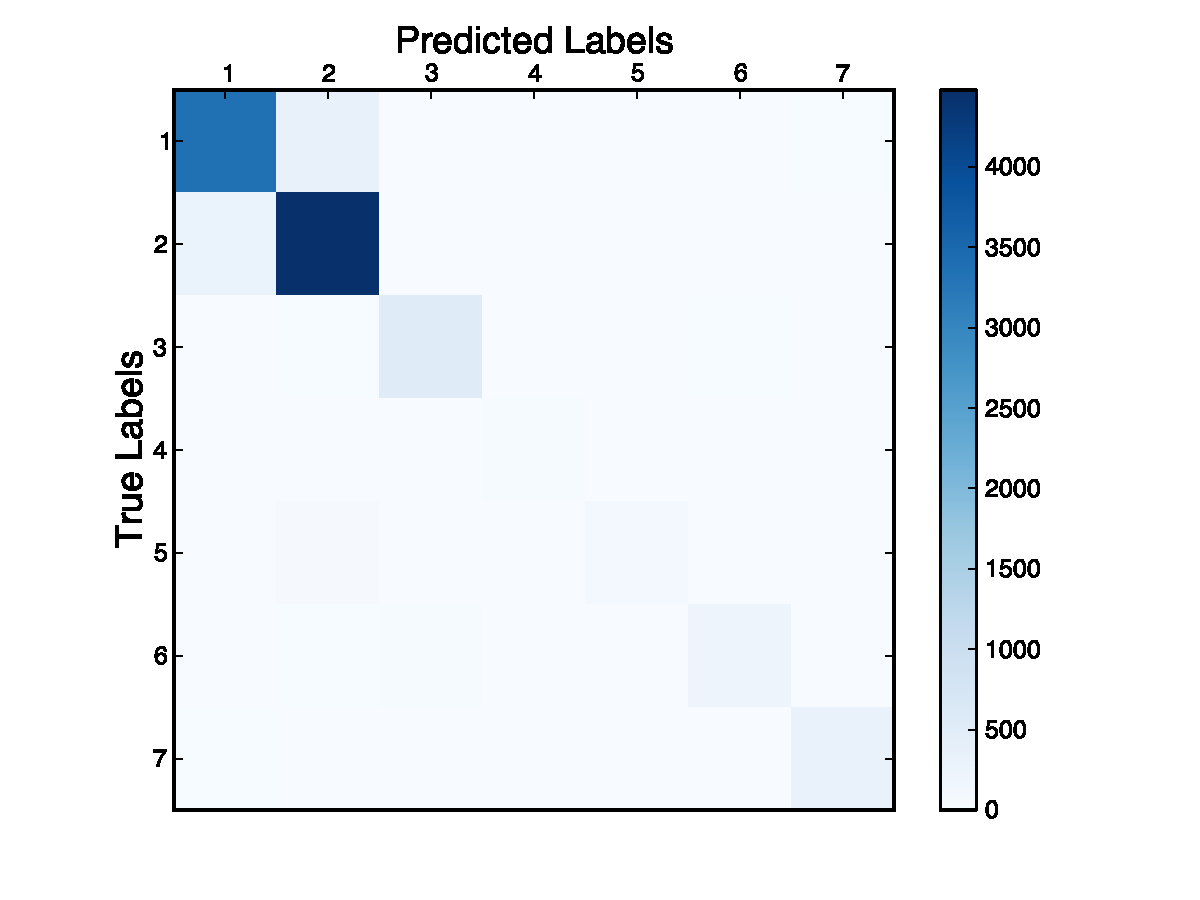
\includegraphics[scale=0.55]{extra_trees_cm.pdf}
\caption{Confusion Matrix for Extra Trees}
\label{fig:extra}
\end{figure} 

As can be seen in the matrix, most of the error in the model stems from confusion between classes 1 and 2 (Spruce/Fir and Lodgepole Pine, respectively).  In order to reduce some of this error, I decided to look for features which seemed to emphasize the difference between these two classes.  Feature 0 (Elevation), shown below, seemed to provide the most hope for increasing separation.  

\begin{figure}[!ht]
\centering
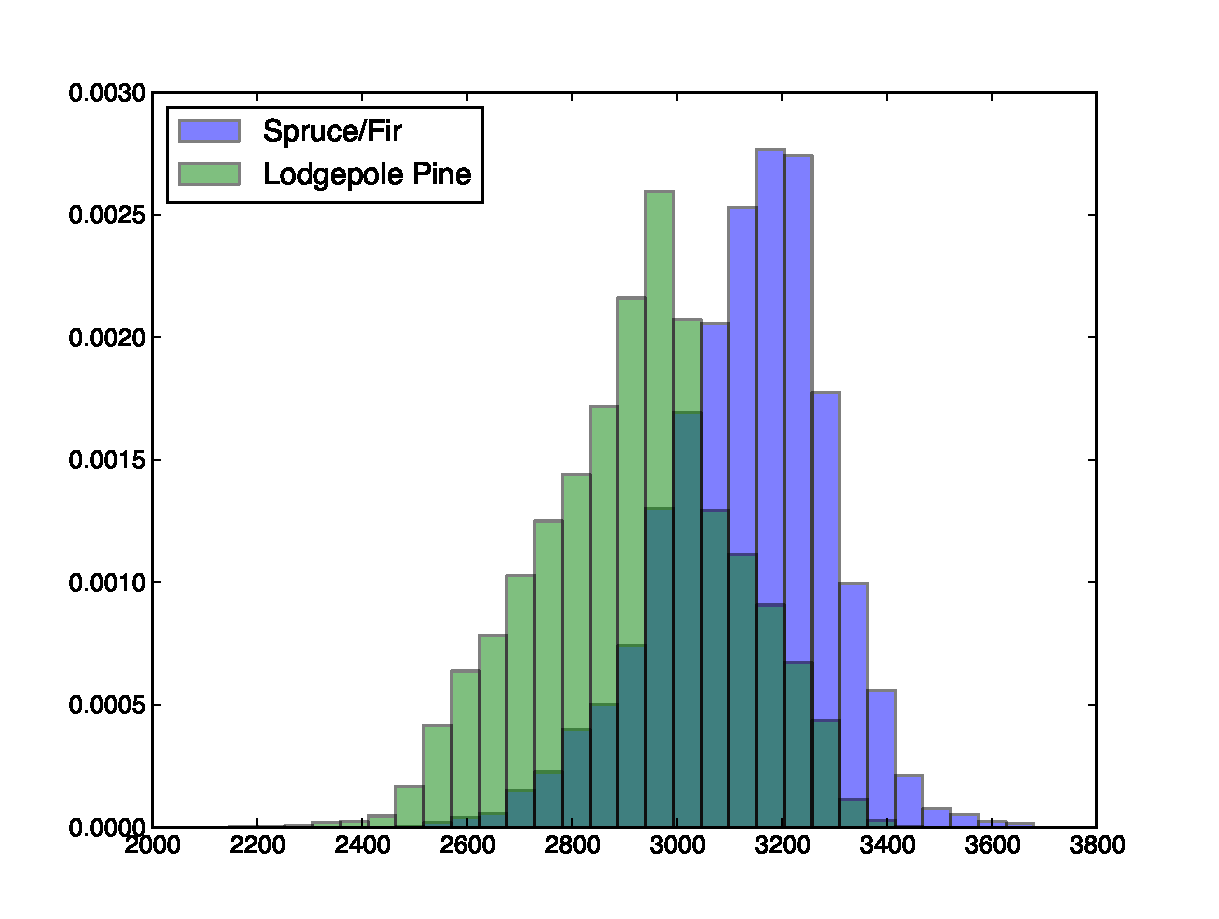
\includegraphics[scale=0.5]{feature0.pdf}
\caption{Elevation for two frequently mistaken classes of cover type}
\label{fig:extra}
\end{figure} 

Unfortunately, my efforts to manufacture additional features (squaring, above/below set threshold, etc.) provided little to no improvement in classification accuracy. 

\section*{Final remarks}

My final model was an Extremely Randomized Trees classifier (Extra Trees algorithm) with 1000 estimators (trees), with a maximum of 10 features considered at each split.  Splits were chosen based on information gain.  This model, paired with a preprocessing step which scaled all input to the range of [0,1], produced my best classification accuracy (91.976\%), which at the time of writing this was near the top of the leader board.   

\section*{Extra information}
\subsection*{Parameter searches}

To select model parameters, I used scikit-learn's GridSearchCV class, found in the \verb!grid_search! module.  For SVM, I searched across several kernel methods (linear, RBF, sigmoid, poly) and a range of C values (1, 10, 100, 1000), and gamma (0.001, 0.0001).  For Random Forests and Extremely Randomized Trees, I performed a grid search to select the number of estimators (50, 100, 500, 1000, 2000), the splitting criterion (entropy versus gini), the maximum number of features to select (5, 9, 10, 12), and whether or not to bootstrap samples.  

\subsection*{Code repository}

In case it's easier to look at this way, I backed up my project to Github:\\ \url{https://github.com/samfway/trees}

\bibliographystyle{unsrt}
\bibliography{References}

\end{document}

